% mainDoc.tex - Main part of the document

\nonumsection*{ABSTRACT}\addcontentsline{toc}{section}{ABSTRACT}

\fishname (\emph{\sciencename}, Turbot) is an important component of the trawl fishery in British Columbia, and are caught ubiquitously along the west coast of British Columbia (Figure~\ref{fig:cpue}).

\newpage	%French abstract must appear on new page

% \section*{R\'esum\'e}\addcontentsline{toc}{section}{R\'ESUM\'E}
\nonumsection*{R\'ESUM\'E}\addcontentsline{toc}{section}{R\'ESUM\'E}

% \addcontentsline{toc}{section}{R\'ESUM\'E}

\clearpage

% Need numbering back to Arabic.
\pagenumbering{arabic}
\setcounter{page}{1}

\section{INTRODUCTION}

This stock assessment is for Arrowtooth Flounder in combined Pacific Marine Fisheries Commission (PMFC) major areas 3CD and 5ABCDE off the west coast of British Columbia. \fishname make up a large component of the trawl fishery, but most are and have been discarded at sea. Proteolysis occurs in the muscle tissue of this species a short time after it is caught, which makes the flesh very mushy and unpalatable. There is a market in Korea for the frills, and a market for the fillets if they are frozen at sea, very shortly after capture.

\subsection{Purpose of Document}

This document provides stock assessment advice to fisheries managers for Arrowtooth Flounder. This advice was requested by the Groundfish Management Unit (GMU) of the DFO Pacific Region (Appendix A), which specified that the advice be framed in terms of the DFO Sustainable Fisheries Framework (SFF) (see \citet{dfo09}). This advice is presented as a set of decision tables that provide probabilities of exceeding reference points over a range of projection years and across a range of constant catch scenarios (without feedback controls). Reference points are defined below.

CITETEST: \citet{arf1995}, \citet{arf1999a}, \citet{arf1999b}, \citet{arf2000}, \citet{arf2001}, \citet{arf2003}, \citet{arf2006},\citet{arf2013}.

\subsection{BIOLOGICAL BACKGROUND}

Arrowtooth Flounder (\emph{Atheresthes stomias}, Turbot) is a species of flatfish found along the rim of the Northeast Pacific Ocean. The most distinguishing feature of Arrowtooth Flounder is its large teeth, for which it was named. As juveniles smaller than ~380mm, Arrowtooth Flounder are monomorphic. After maturing, they are sexually dimorphic with adult females being larger than males (Appendix~\ref{chap:biological}, Figure~\ref{fig:vonb}).

\subsection{RANGE AND DISTRIBUTION}


\subsection{OVERVIEW OF FISHERY}


\section{ASSESSMENT BOUNDARIES AND BACKGROUND}

For this assessment, we use PMFC major areas 3CD and 5ABCDE, covering almost all of the west coast of Vancouver Island (Figure~\ref{fig:areas}).

Advice for managers was requested to be guided by the DFO Sustainable Fisheries Framework, particularly the Fishery Decision-making Framework Incorporating the Precautionary Approach. Consequently, advice to managers is presented as a set of decision tables that provide probabilities of exceeding reference points for various years of projections across a range of constant catch scenarios.

A DFO Technical Working Group provided valuable guidance with respect to many of the decisions that were made in the course of this work.

\section{CATCH DATA}
*Table with history of quota and catch from 1996-present

\section{FISHERIES MANAGEMENT}

\clearpage

\section{SURVEY DESCRIPTIONS}

Six sets of fishery independent survey indices of abundance were used:

\begin{enumerate}[noitemsep,nolistsep]
  \item the West Coast Vancouver Island Synoptic Survey series, from 2004-2014 (even years only), referred to here as the `WCVISS series'.
  \item the Hecate Strait Synoptic Survey series, from 2005-2013 (odd years only), referred to here as the `HSSS series'.
  \item the Hecate Strait Multispecies Assemblage Survey, for 1996, 1998, 2000, 2002, and 2003, referred to here as `HSMAS'.
  \item the West Coast Vancouver Island Shrimp Trawl Survey, from 1996-2014 (all years), referred to here as `WCVISTS'.
  \item the Queen Charlotte Sound Synoptic Survey, from 2003-2013 (odd years only), referred to here as `QCSSS'.
  \item the Queen Charlotte Sound Shrimp Trawl Survey, from 1999-2013 (all years), referred to here as `QCSSTS'.
\end{enumerate}

The suitability of each survey was examined (Table~\ref{tab:surveySuitability}). The WCVISS, HSSS, HSMSAS, and QCSSS were all designed to produce indices for the demersal fish species of the Northeast Pacific, and the two shrimp trawl surveys WCVISTS and QCSSTS were designed to generate shrimp indices. The depth ranges differ by a large amount, with the 4 groundfish surveys having ranges from 18 m to 660 m. The shrimp trawl surveys have a maximum depth of 251 m and 305 m for the WCVISTS and QCSSTS respectively (Table~\ref{tab:surveySuitability}). The depth range for \fishname\ is 50 m to 900 m (\citet{arf2001}); the shrimp trawl surveys cover much less of the habitable depth range than the groundfish surveys do, 

suggesting that they might not be suitable as an index of stock for

The relative biomass survey indices are used as data in the model along with the associated relative error for each index value.

Pre-1996 commercial catch and effort data were also investigated with the intent of creating CPUE-based abundance indices for use in the stock assessment model. This approach was abandoned because it was felt that there were problems with the reliability of the data as well as questions as to the representative nature of the resulting indices, given the schooling behaviour of the species and the capacity of fishers to target these schools. Given the concern that the resulting indices would be hyperstable, they were not used in this assessment.

\clearpage

\section{BIOLOGICAL INFORMATION}

\subsection{BIOLOGICAL SAMPLES}

\subsection{GROWTH PARAMETERS}

\subsection{MATURITY}

\subsection{NATURAL MORTALITY}

PAST ASSESSMENTS have assumed M.... etc.. cite Fargo Starr and Alaska center assessments. Very sensitive to assumptions in the model iscam.

Male and female natural mortalities were estimated as parameters of the model (see Appendix~F), using an informed prior based on the marginal posterior distributions from the QCS POP assessment , specifically a normal prior with mean 0.07 and standard deviation 0.007 for both sexes (see Appendix~F). The QCS assessment used a prior based on a POP assessment for the Gulf of Alaska , with mean 0.06 and standard deviation 0.006.

In recent assessments , model runs that fixed natural mortality were also used to provide the final advice to managers. However, because we were able to develop a prior based on Canadian POP data, and since the resulting Bayesian estimates of natural mortality and steepness (defined below) are uncorrelated (Appendix~G), only runs that estimate natural mortality are used in this assessment (as agreed upon by the Technical Working Group). Prior distributions for all estimated parameters are given in Table F.4.

\section{AGE-STRUCTURED MODEL}

We attempted a two-sex, age-structured stochastic model to reconstruct the population trajectory of Arrowtooth Flounder
*Reference Appendix for model outputs and sensitivities...

REASONS model was rejected.

\section{RESULTS}

MOVE TO APPENDIX FOR MODEL RESULTS
THIS IS ALL POP!!!!!!!!!!!!!!!!!!!!!!!!!!
The base case model run had credible fits to the data, as demonstrated by visual examination of the MPD fits and the patterns of residuals (results in Appendix G). The MCMC results showed satisfactory convergence of the MCMC search process (Appendix G). Priors and marginal posteriors of the estimated parameters are also given in Appendix G, along with the values of the estimated parameters (Table \ref{tab:MCMCpar}). For example, natural mortality is estimated as having median (and 5-95\% credible interval) of 0.069~(0.060-0.079) for females and 0.072~(0.063-0.082) for males. Steepness is estimated to be 0.70~(0.48-0.91). The remaining MCMC results, of more general interest, are given here.

Figure \ref{fig:VBcatch} shows the MCMC results for the estimated vulnerable biomass, together with the reconstructed historical catches, and Figure \ref{fig:BVBnorm} shows the estimated medians of vulnerable and spawning (mature females only) biomass relative to their unfished values. (The full MCMC results for spawning biomass are included later in Figure \ref{fig:Bproj} regarding projections). These demonstrate a slight decline in biomass from 1940 to 1960 with the onset of fishing, followed by a very sharp decline in the 1960s due to heavy fishing (primarily by foreign fleets). After the cessation of foreign fishing, the biomass increased through the remainder of the 1970s. The biomass then declined through the 1980s until the mid-1990s, and has since increased, with median values of relative biomass now above the 1980 values.

Estimates of various quantities of interest are given in Table \ref{tab:MCMCderived}. In particular, the median (and 5-95\% credible interval) for $B_{2013}/B_0$, the ratio of current spawning biomass ($B_{2013}$) to the unfished equilibrium level ($B_0$), is 0.41~(0.19-0.68); thus 0.41 is the value for the final circle in Figure \ref{fig:BVBnorm}.
% (This ratio is sometimes known as depletion).

The estimated recruitments (age-1 fish, Figure \ref{fig:recruitsMCMC}) in part further explain the aforementioned stock trajectory. There was lower-than-average recruitment in the early 1970s, which may, together with increased catches, explain why the vulnerable biomass declined through the 1980s (note the approximate ten-year lag from recruitment to fish becoming fully selected by the commercial fishery). There are a number of year classes with approximately double the long-term average recruitment. This is unlike the patterns observed for the QCS area 5ABC stock (Figure 5 of  and the companion assessment for area 5DE , which both exhibited a dominant 1976 year class (age-1 recruits in 1977) that was approximately five times larger than the long-term average recruitment.

Figure \ref{fig:exploitMCMC} shows the estimated exploitation rates (ratio of total catch to the vulnerable biomass in the middle of the year), which peaked in the mid-1960s due to the large foreign catches, and then peaked again (although not as high) in the early 1990s due to increased domestic exploitation. Exploitation rates have remained low since the mid-1990s, with $u_{2012}$, the exploitation rate for 2012, estimated to be 0.035~(0.018-0.077).

Estimates of further quantities of interest, such as absolute values of biomass (rather than relative values), are also given in Table \ref{tab:MCMCderived}, as well as quantities based on MSY, discussed below.

\section{RECCOMENDATIONS AND YIELD OPTIONS}

\subsection{CURRENT STOCK LEVEL}

\subsection{REFERENCE POINTS}

\subsection{PROJECTION RESULTS AND DECISION TABLES}

\section{GENERAL COMMENTS}

\section{FUTURE RESEARCH AND DATA REQUIREMENTS}

\section{ACKNOWLEDGEMENTS}

We thank the members of the Arrowtooth Flounder Technical Working Group (Rowan Haigh, Kendra Holt, Rob Kronlund, Barry Ackerman, Greg Workman) for their valuable advice as this project progressed. We thank participants of the Regional Peer Review meeting for their comments at the meeting, and Rowan Haigh for chairing. We especially thank James Thorsen (NOAA) and Joanne Morgan (DFO) for their written reviews of the working paper. We also thank Steve Wischniowski and the members of the Sclerochronology Laboratory at the Pacific Biological Station for their processing of over 6,000 Arrowtooth Flounder otoliths in 2014.

\addcontentsline{toc}{section}{BIBLIOGRAPHY}
\bibliographystyle{resDoc}
\bibliography{../../all}

\clearpage

\begin{figure}[htp]
\begin{center}
\includegraphics[width=6in,keepaspectratio=true]{cpueFigures/ARF-1996-2014-CPUE.eps}
\end{center}
\vspace{0mm}
% To get the grid size in km^2 for the caption:
% While in the gui for the map, type mean(xtcall(PBSmap)$pdata$area) for the map you currently have loaded.
\caption{Mean catch-per-unit-effort (CPUE, kg/h) of Arrowtooth Flounder in grid cells 0.1$^\circ$ longitude by 0.075$^\circ$ latitude (roughly 57.8~km$^2$). The shaded cells give an approximation of the area where Arrowtooth Flounder was encountered by fishing events from the groundfish trawl fishery from January 1, 1996 to October 7, 2014. Contours are 200 m and 1000 m isobaths. Red lines are PFMA area boundaries.}
\label{fig:cpue}
\end{figure}

\begin{table}[b]
\tiny
\centering
\caption{\label{tab:surveySuitability} Attributes of fishery-independent surveys and evaluation of suitability for stock indexing. RS=Random stratified design, BT=Bottom trawl gear.}
\begin{tabular}{lcccccc}
\hline
Attribute                &        WCVISS &          HSSS &         HSMSAS &         QCSSS &        WCVISTS &         QCSSTS \\
\hline
Design                   &            RS &            RS &             RS &            RS &             RS &             RS \\
Gear                     &            BT &            BT &             BT &            BT &             BT &             BT \\
Year Range (years)       & 2004-2014 (6) & 2005-2013 (5) & 1984-2003 (11) & 2003-2013 (7) & 1977-2014 (38) & 1998-2013 (16) \\
Set Range (avg)          & 106-179 (153) & 156-236 (189) &   88-161 (105) & 260-281 (269) &   67-204 (131) &   92-204 (175) \\
PFMA Areas               &         3C,3D &         5C,5D &          5C,5D &         5A,5B &          3C,3D &          5A,5B \\
Depth Range (m)          &        41-660 &        19-420 &         18-232 &        41-626 &         15-251 &         15-305 \\
Ageing done (yrs)        &       Yes (5) &       Yes (5) &        Yes (1) &            No &             No &             No \\
Comment                  &               &               &                &               & \specialcell{Targets\\shrimp} & \specialcell{Targets\\shrimp} \\
\hline
\end{tabular}
\end{table}


\clearpage
